\chapter{Background}

According to seminal research by \cite{krizhevsky2012imagenet}, lorem ipsum dolor sit amet. However, this result was already known in the 1990s \cite{lecun1998gradient}. 

\section{Structure and Layout}

Reports written for scientific works, such as degree theses, should feature a specific structure and layout according to well-established standards, which also apply to professional publications of any kind.

In particular, degree theses should have the following contents:
\begin{itemize}
	\item Title page;
	\item Abstract;
	\item Table of contents;
	\item List of symbols (optional);
	\item List of abbreviations (optional);
	\item List of figures (optional);
	\item List of tables (optional);
	\item Text of the thesis, roughly structured as:
	\begin{itemize}
		\item Introduction;
		\item Body;
		\item Conclusion;
	\end{itemize}
	\item Bibliography;
	\item Appendix (optional).
\end{itemize}

An essential aspect is the effective transfer of written information to an educated reader who is not directly familiar with the problem. This includes:
\begin{itemize}
  \item A clear presentation of the evolution of thoughts from the level of knowledge at the beginning of the work to the developed solution;
  \item A good structure and a logical arrangement;
  \item An understandable, short, and exact formulation without deviating from the topic.
\end{itemize}

The level of knowledge is given by the results of preliminary studies and previous publications. Proposals for the problem's solution must be discussed, and the chosen approach has to be justified. Fundamental analysis that does not lead to success must be added with an explanation. The structure and order of the text are based on objective criteria, not on the temporal sequence of development. Subheadings should be well chosen. Frequent hints about the path followed place the sections in context.

The description of the studies and experiments must be detailed enough to allow for replication by others. The results must be reproducible. All tools, such as literature, formulas, programs, or measurement methods, must be indicated. The results or solutions adopted should be explained only to the extent necessary for understanding, with reference to the source but without derivation.

Often, measured and calculated results and functional correlations can be displayed more clearly and understandably with figures or tables than with long descriptions. It is assumed that extensive mathematical derivations or proofs are listed in one or more appendices, as well as collections of figures or tables that break the context of a text passage. The text must include references to all parts of the thesis (figures, tables, literature, attachments).

\subsection{Structure}

\subsubsection{Title Page}

The layout of the title page is given by a template, according to the title page of this guide.

\subsubsection{Table of Contents}

The table of contents consists of the numbered headings of the sections and the corresponding first page numbers. Appendices must also be listed. Page numbering should start with the table of contents as page 1.

Attention should be paid to the consistent capitalization of the headings in the table of contents. Unclear and uncommon abbreviations should be avoided in the headings.

\subsubsection{List of Symbols}

A list of symbols should be provided if the thesis contains many formulas. All symbols used must be arranged alphabetically and described briefly.

\subsubsection{List of Acronyms}

A list of acronyms should be provided if the thesis contains many acronyms, especially within graphics and diagrams. In this list, only uncommon acronyms should be given in alphabetical order and should be briefly described.

\subsubsection{Bibliography}

All sources of information used must be cited in the thesis and listed in the bibliography. In brackets are the reference numbers of the citations. The order of numbering of the cited sources must be that of the first appearance of the citations in the text. When referring to multiple sources, consideration of standardization and uniformity of symbols and abbreviations is required. If necessary, the symbols and abbreviations of the cited sources should be adapted to match the entries in the list of symbols and abbreviations in the thesis. The reference to sources from the Internet is allowed only in special cases, given the vicissitude and transience of these sources. Verify the accuracy of all references, even if taken from other (intermediate) sources.

\subsubsection{Appendix}
\label{sec:appendix}

The appendices of a thesis should be numbered. Each appendix contains the following introductory information:
\begin{itemize}
  \item Appendix A (consecutively letter);
  \item Title of the appendix;
  \item Index of the appendix (only when the relevant appendix needs structuring due to length).
\end{itemize}

The following components of a thesis should generally be part of the appendices rather than of the report:
\begin{itemize}
  \item Documentation used in the work, such as program lists and scripts, flowcharts, descriptions of programs, and user information;
  \item Documents related to devices that have been constructed during the work, such as circuit diagrams, layout diagrams, and instruction sheets.
\end{itemize}

\subsubsection{Statements}

Based on the results and conclusions of the work, short and precise statements should be provided, aimed at the educated reader and encouraging scientific discussion.

\subsection{Text Layout}

\subsubsection{Structure}

The decimal numeration of the sections generates the structure of the text. Every section of text must have a headline.

\subsubsection{References}

References in the text to other sections are preferably specified by the corresponding page number. References of figures, tables, and equations must be identified by the source index. These references should be inserted either near the point of the sources in the text or indicating the page number. Literature references should be arranged according to their index number in the bibliography. These citation numbers must appear in the continuous text, not as footnotes. Footnotes should be avoided whenever possible.

\subsubsection{Citations}

The citation of external sources has several purposes:
\begin{itemize}
	\item To support intellectual honesty (and avoid plagiarism), since extrinsic ideas should be marked as such; and
	\item To confirm the data and facts the work is based on.
\end{itemize}

If, in a thesis, reference is made to specific data, facts, or texts, the source must also be mentioned. A pure statement of a fact without citing a source is not admissible. However, a reference is not necessary if the asserted statement is an accepted matter of fact in the particular field.

Several types of citations can be distinguished:
\begin{enumerate}
	\item Direct citations
	
	The verbatim copying of external text parts into the own thesis is referred to as a direct citation. It is used to analyze or interpret the statement of the cited source. For a direct citation, the following points should be observed:
\begin{itemize}
	\item The citation must be placed in quotation marks;
	\item The source must be cited literally;
	\item The reference to the source follows at the end of the cited text part;
	\item Text parts in a foreign language should be cited in the original language. They should be amended by a translation that is put in parentheses;
	\item Own annotations or changes within the citation should be marked with square brackets. Optional omissions should be marked with square brackets and ellipsis.
\end{itemize}

Citations that are longer than three lines can be indented as a block. In this case, no quotes are used.

Example:
\begin{quote}
	This is a long and more comprehensive citation from a certain source that fills several text lines. It is indented as a block in the running text to be referred to as a more extended citation.
\end{quote}

In many cases, not only the content but also the style of a citation is essential. Therefore a direct citation should also copy a particular emphasis of the text (e.g., italics, bold text) and the exact punctuation.

	\item Indirect Citations

	The analogous adoption of external text parts or imitation with respect to the content is denoted as an indirect citation. It is used to support one's explanations and positions. Indirect citations are not put into quotation marks. The reference to the source follows the respective text part.
\end{enumerate}

Direct and indirect citations can be documented with the exact page number of the source. The references link to the bibliography. Therefore the following notation can be used:
\begin{itemize}
	\item The page number can be mentioned inside the square brackets for a direct or indirect citation.
	
	Example: This is a direct citation~\cite[p.~4]{lecun1998gradient}.
	
	Example: This direct citation [\ldots] spans two pages~\cite[p.~4 f.]{lecun1998gradient}.
	\item If the source ranges over three or more pages, the exact page range should be specified.
	
	Example: This indirect citation refers to a longer passage~\cite[p.~4--8]{lecun1998gradient}.
	
	\item If several short sources (e.g., articles) are cited thoroughly, the references can be directly grouped.
	
	Example: This relation is described in more detail in~\cite{krizhevsky2012imagenet,lecun1998gradient}.
\end{itemize}

\subsubsection{Acronyms}

Common acronyms can be used without explanation; others need to be explained when they first appear in the text. The acronyms used in text and graphics must be consistent.

\subsubsection{Symbols and Units}

The International System of Units must be considered for the choice of units. Every symbol must be well-defined when it first appears. Symbols used in text and graphics must be consistent.

\subsubsection{Equations and Formulas}

Equations and formulas should be written on separate lines. All or at least all important formulas must be numbered in parentheses on the right hand. Equations should be written as quantity equations. If exceptions are needed, numerical values must always provide their corresponding units. 

As an example of correct typesetting and layout, the Pythagorean Theorem is used:
\begin{equation}
	a^2 + b^2 = c^2
\end{equation}

For multi-line equations, the equal signs should be aligned on top of each other.

\section{A Section that Contains a Figure}

Pictures and graphical representations must be labeled with a caption and numbered progressively. The abbreviation ``Fig.'' should be used when referring to specific figures.

Figures that belong together should be placed as sub-figures side by side or one below the other. Sub-figures should be provided consecutively with lower case letters. Figure captions should be self-explanatory. Unclear and uncommon abbreviations should be avoided in the figure caption. Explanations that may be necessary to understand the figure should also be given in the caption, such as the meanings of multiple curves in the same diagram or the necessary boundary conditions under which the curves were obtained. The figure itself should contain the least amount of text possible. If a figure is used that the author did not create himself, the source of the figure should be cited within or at the end of the figure caption directly below the figure. This also applies to figures that have been adapted or changed.

Diagrams, plots, and line graphs should be included as vector graphics. Only photographs should be inserted as a bitmap graphic. The physical quantities displayed in diagrams and plots must be specified with their corresponding unit. The font size of the axis labels and tick marks must be legible (as in the text). Especially in smaller sub-figures, it has to be ensured that the font size is large enough. The scale of a diagram must be chosen in accordance with the accuracy of the quantity presented. The type of grid division (e.g., linear or logarithmic) must be evident. A zero suppression of an axis should be clearly marked with a break of the corresponding axis. Curves of statistically fluctuating measured data may be smoothed. Measured points or sparse data points of low density should be printed with a clear signature, e.g.~by symbols like $+$, $\times$, $\circ$, $\bullet$, or $\ast$.

\begin{figure}[t]
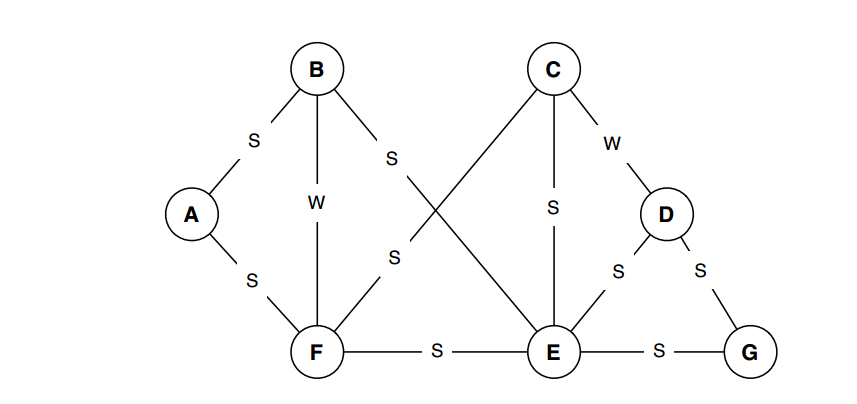
\includegraphics[width=15cm]{figures/figure1.png}
\caption{A simple figure.}
\label{fig:graph}
\end{figure}

Figures should always be placed at the top or bottom of the page they appear on (see Fig. \ref{fig:graph}).

\section{A Section that Contains a Table}

Numerical tables and compilations of data or facts in tabular form must be numbered consecutively. Each table must be labeled with a caption. Each caption should be unique so that two or more tables never share the same caption. The caption must be placed above the table, as it helps the reader to grasp the content of the table, even in the case of a long table running over several pages. Where applicable, the physical quantity listed must be indicated in the header of each column by a formula symbol or word and the corresponding unit.

Tables should always be placed at the top or bottom of the page they appear on or, as in this case, at the end of the section/chapter (see Table \ref{tab:xor}).

\begin{table}[ht!]
\center
\caption{A simple table.}
\begin{tabular}{cc|c}
A & B & A XOR B\\
\hline
0 & 0 & 0\\
0 & 1 & 1\\
1 & 0 & 1\\
1 & 1 & 0\\
\end{tabular}
\label{tab:xor}
\end{table}